% L22eqv.tex
%
% Predrag created file              jul  9 2006
% $Author$ $Date$


\section{Small $L=22$ system {\rpo s}}
\label{s:L22}
\file{L22eqv.tex}


\KS\ system with $L = 22$ periodic on the full space is small but
empirically large enough to exhibit persistent chaos.  $L=22$ is a
sensible choice because in units of mean wavelength the size of this
small system is about 2.5 wavelengths ($\tildeL/\sqrt{2}= 2.4758$),
so the dynamics is a competition between wavenumbers 2 and 3.
Because of the strong $k^4$ contraction in \KS\ we expect a small
number of eigenvalues to be significant for the dynamics, while the
rest are in the numerical noise. See figure~6 in
\refref{Christiansen:97}.

%% Davidchack and Crofts
% We investigate this system in 16 to 64 complex Fourier modes (32 to
%128-dimensional system of real ODEs) truncation, and recheck the results
%by redoing the calculation with the double number of Fourier modes. %
%observe how many digits change. The \eqv\ points are accurate to at least
%to $10^{-11}$. Since Lapack is also double precision accurate, the
%accuracy of the first few eigenvalues is similar, and certainly in excess
%of 6 significant digits. % All digits stated in tables are significant.
%The accuracy that can be reached is of order of
%$|a(\period{p},d_p) - a_0|
% \approx \epsilon \exp(\Lyap_p \period{p})$,
% where $\epsilon \approx 10^{-17}$ for double precision, $\Lyap_p$ is
%the largest Lyapunov exponent, and $\period{p}$ the period.  With a good
%starting guess, Newton's method typically reaches that accuracy after 2-3
%iterates.

\subsection{\Eqva}

In addition to the trivial equilibrium $u=0$ (denoted E0 from now
on), we find for $L = 22$ three \eqva\ with dominant wavenumber $k$
(denoted E$k$) for $k = 1, 2, 3$.  All equilibria, shown in
Fig.~\ref{f:KS22Equil}, are symmetric with respect to the reflection
symmetry. The \eqva\ E2 and E3 have additional symmetry with respect
to translation by $L/2$ and $L/3$, respectively.

\begin{figure}[h]\vspace*{-5pt}
\centering
(a)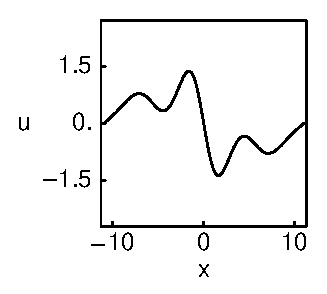
\includegraphics[width=0.25\textwidth]{figs/1wKS22equil.eps}
(b)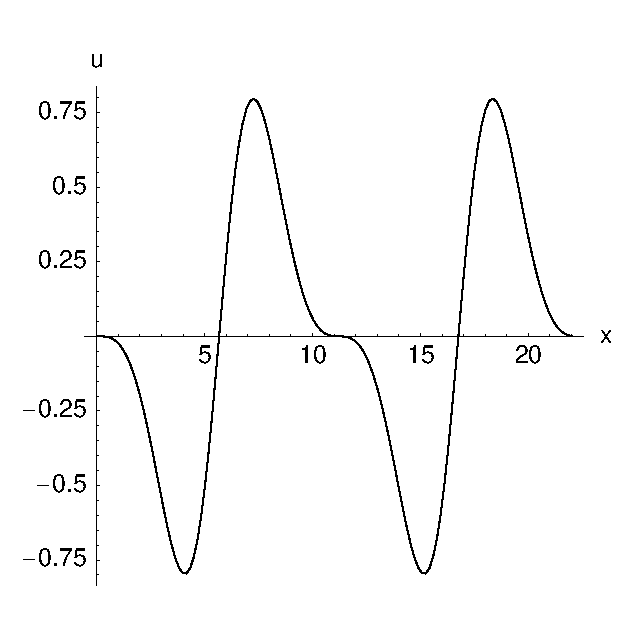
\includegraphics[width=0.25\textwidth]{figs/2wKS22equil.eps}
(c)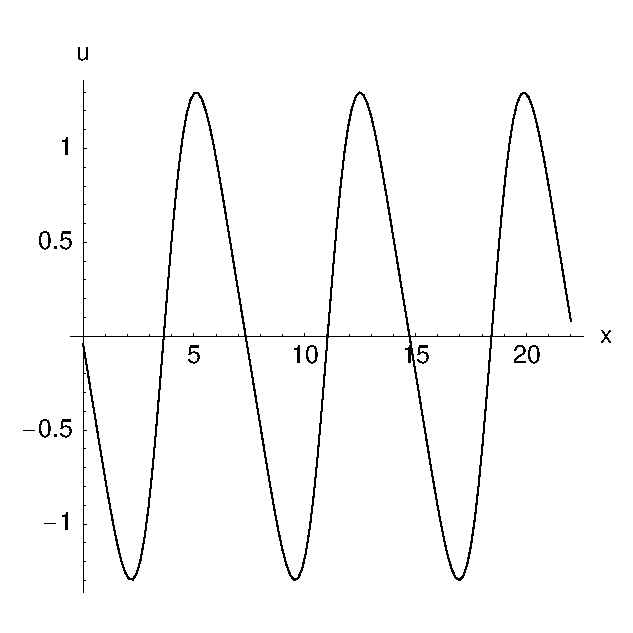
\includegraphics[width=0.25\textwidth]{figs/3wKS22equil.eps}
\vspace*{-5pt}\caption{ {\small (a) E1, (b) E2 and (c)
E3~\eqva\ of \KS\ equation with $L=22$.}}
\label{f:KS22Equil}\vspace*{-5pt}
\end{figure}

%\begin{figure}
%  \includegraphics[width=12cm]{figs/L22-E123.eps}\\
%  \caption{\KSe\ equilibria for $L=22$.}\label{fig:E123}
%\end{figure}

The stability of the equilibria is characterized by the eigenvalues
$\lambda_j$ of the Jacobian matrix.  First ten eigenvalues for each
equilibrium are listed in Table~\ref{tab:Ek_eigs} in the order of
decreasing real parts. Recall that an equilibrium with $\mathrm{Re}
\lambda_j > 0$ is unstable in the direction of the corresponding
eigenvector $e_j$.

\begin{table}
\caption{\label{tab:Ek_eigs} Eigenvalues of the \eqva\ for $L=22$.}
{\small
\begin{tabular}{cccc} \hline
  E0       &        E1         &         E2        &     E3   \\\hline
  $0.2198$ &  $0.1308+i0.3341$ &  $0.1390+i0.2384$ &  $0.0933$\\
  $0.2198$ &  $0.1308-i0.3341$ &  $0.1390-i0.2384$ &  $0.0933$\\
  $0.1952$ &  $0.0824+i0.3402$ &  $0$              &  $0$\\
  $0.1952$ &  $0.0824-i0.3402$ & $-0.0840+i0.1602$ & $-0.4128$\\
  $0.0749$ &  $0$              & $-0.0840-i0.1602$ & $-0.6108+i0.3759$\\
  $0.0749$ & $-0.2287+i0.1963$ & $-0.1194$         & $-0.6108-i0.3759$\\
 $-0.3981$ & $-0.2287-i0.1963$ & $-0.2711+i0.3563$ & $-0.6108+i0.3759$\\
 $-0.3981$ & $-0.2455$         & $-0.2711-i0.3563$ & $-0.6108-i0.3759$\\
 $-2.1191$ & $-2.0554$         & $-2.0130$         & $-1.6641$\\
 $-2.1191$ & $-2.0619$         & $-2.0378$         & $-1.6641$\\\hline
\end{tabular}}
\end{table}

The eigenvalues of E0 are determined by the linear part of the \KS\
equation: $\lambda_k=q_k^2-q_k^4$, where $q_k = 2\pi k/L$.  For
$L=22$, there are three pairs of unstable eigenvalues: corresponding
to three unstable modes $k=2,3$, and 1, respectively.  For each
mode, the corresponding eigenvectors lie in the plane spanned by
$\mathrm{Re} a_k$ and $\mathrm{Im} a_k$. Tables \ref{tab:E1_sym} to \ref{tab:E3_sym}
list the symmetries corresponding to the stability eigenvectors of \eqva E1-E3.
With $S$, $A$ we denote an eigenvector belonging to the symmetric
or antisymmetric subspace respectively. The last column lists
the symmetry expected to be present in the corresponding
stable/ustable manifold.

\begin{table}[h!]
\caption{\label{tab:E1_sym} Symmetries of eigenvectors of E1 for $L=22$.}
{\small
\begin{tabular}{cccc} \hline
          $\lambda_i$       & $\mathrm{Re}(e_i)$    & $\mathrm{Im}(e_i)$    & $\mathcal{M}$ \\\hline
    $0.1308 \pm i0.3341$    & S     & S     & - \\
    $0.0824 \pm i0.3402$    & A     & A     & A \\
    $0$                     & S     &       & - \\
    $-0.2287+i0.1963$       & A     & A     & A \\
    $-0.2455$               & S     &       & - \\
    $-2.0554$               & A     &       & A \\
    $-2.0619$               & S     &       & - \\\hline
\end{tabular}}
\end{table}

\begin{table}[h!]
\caption{\label{tab:E2_sym} Symmetries of eigenvectors of E2 for $L=22$.}
{\small
\begin{tabular}{cccc} \hline
          $\lambda_i$       & $\mathrm{Re}(e_i)$    & $\mathrm{Im}(e_i)$    & $\mathcal{M}$ \\\hline
      $0.1390\pm i0.2384$   & A     & A     & A \\
      $0$                   & S     &       & - \\
      $-0.0840\pm i0.1602$  & S     & S     & - \\
      $-0.1194$             & S     &       & - \\
      $-0.2711\pm i0.3563$  & A     & A     & A \\
      $-2.0130$             & S     &       & - \\
      $-2.0378$             & A     &       & A \\\hline
\end{tabular}}
\end{table}

\begin{table}[h!]
\caption{\label{tab:E3_sym} Symmetries of eigenvectors of E3 for $L=22$.}
{\small
\begin{tabular}{cccc} \hline
          $\lambda_i$    & $\mathrm{Re}(e_i)$    & $\mathrm{Im}(e_i)$    & $\mathcal{M}$ \\\hline
    $0.0933$             &  A    &       & A \\
    $0.0933$             &  S    &       & - \\
    $0$                  &  S    &       & - \\
    $-0.4128$            &  A    &       & A \\
    $-0.6108\pm i0.3759$ &  A    &   A   & A \\
    $-0.6108\pm i0.3759$ &  S    &   S   & - \\
    $-1.6641$            &  S    &       & - \\\hline
\end{tabular}}
\end{table}


\subsection{Unstable invariant manifolds of \eqva\ and heteroclinic
connections}

In this section we explore the structure of unstable invariant
manifolds of the equilibria.  The E1 equilibrium has two unstable
planes within which the solutions are spiralling out (i.e., two
pairs of complex conjugate eigenvalues).  The E2 has one such plane,
while the E3 has two real positive eigenvalues, so the solutions are
moving radially away from the equilibrium within the plane spanned
by the corresponding eigenvectors.  Since E1 has larger unstable
subspace, it is expected to have much less influence on the system
evolution compared to E2 and E3.

\begin{figure}[h]\vspace*{-5pt} \centering
\includegraphics[width=0.45\textwidth]{figs/ks22_E1_plane1_manifold.eps}
\includegraphics[width=0.3\textwidth]{figs/ks22_E1_plane1_orbits.eps}
\vspace*{-5pt}\caption{ {\small The upper panel shows the unstable
invariant manifold of equilibrium E1 starting within the plane
corresponding to the first pair on unstable eigenvalues. The
coordinate axes $v_1$, $v_2$, and $v_3$ are constructed from vectors
$\mathrm{Re} e_1$, $\mathrm{Im} e_1$, and $\mathrm{Re} e_6$
by Gram-Schmidt orthogonalization.
The lower panel shows spacial representation of two orbits A and B.
The change of color from blue to red indicates increasing values of
$u(x)$.}} \label{f:KS22E1man1}\vspace*{-5pt}
\end{figure}

To construct an invariant manifold containing solutions
corresponding to the pair of unstable complex conjugate eigenvalues,
$\lambda = \sigma\pm i\omega$, $\sigma > 0$, we start with a set of
initial conditions near equilibrium $a_{\mathrm{E}k}$:
\[ a(0) = a_{\mathrm{E}k} + \epsilon\,v\mathrm{e}^{\delta}\]
where $\delta$ takes the set of values uniformly distributed in the
interval $[0,2\pi\sigma/\omega]$, $v$ is a unit vector in the
unstable invariant plane, and $\epsilon > 0$ is small.

\begin{figure}[h]\vspace*{-5pt} \centering
\includegraphics[width=0.45\textwidth]{figs/ks22_E1_plane2_manifold.eps}
\includegraphics[width=0.45\textwidth]{figs/ks22_E1_plane2_orbits.eps}
\vspace*{-5pt}\caption{ {\small The upper panel shows the unstable
invariant manifold of equilibrium E1 starting within the plane
corresponding to the second pair on unstable eigenvalues. The
coordinate axes $v_1$, $v_2$, and $v_3$ are constructed from vectors
Re $e_3$, Im $e_3$, and Re $e_6$ by Gram-Schmidt orthogonalization.
The lower panel shows spacial representation of three orbits. Orbits
B and C pass close to the equilibrium E3.}}
\label{f:KS22E1man2}\vspace*{-5pt}
\end{figure}

The manifold starting within the first unstable plane of E1, with
eigenvalues $0.1308\pm i0.3341$, is shown in
Figure~\ref{f:KS22E1man1}. It appears to fall directly into the
chaotic attractor.  The behaviour of the manifold starting within
the second unstable plane of E1 (eigenvalues $0.0824\pm i0.3402$) is
remarkably different: as can be seen in Figure~\ref{f:KS22E1man2},
all orbits within the manifold converge to the equilibrium E2.  The
manifold also contains a heteroclinic connection from E1 to E3.

\begin{figure}[h]\vspace*{-5pt} \centering
\includegraphics[width=0.45\textwidth]{figs/ks22_E2_manifold.eps}
\includegraphics[width=0.45\textwidth]{figs/ks22_E2_orbits.eps}
\vspace*{-5pt}\caption{ {\small The upper panel shows the two-dimensional
unstable invariant manifold of equilibrium E2. The coordinate axes
$v_1$, $v_2$, and $v_3$ are constructed from vectors
Re $e_1$, Im $e_1$, and $e_7$ by Gram-Schmidt orthogonalization.
The lower panel shows spacial representation of three orbits. Orbits
B and C pass close to the equilibrium E3.}}
\label{f:KS22E2man}\vspace*{-5pt}
\end{figure}

The two-dimensional unstable manifold of E2 is shown in
Figure~\ref{f:KS22E2man}.  All orbits within the manifold converge
to E2 shifted by $L/4$.  So this manifold can be viewed as a homoclinic
connection.  It also contains a pair of heteroclinic connections from
E2 to E3.

The equilibrium E3 has a pair of real unstable eigenvalues
equal to each other.  Therefore, within the plane spanned by the
corresponding eigenvectors, the orbits move radially away from
the equilibrium.  In order to trace out the unstable manifold,
we start with a set of initial conditions within the unstable plane
\[ a(0) = a_\mathrm{E3} + \epsilon(v_1 \cos \phi + v_2 \sin \phi)\,,
  \quad\phi\in[0,2\pi]\,, \]
where $v_1$ and $v_2$ are orthonormal vectors within the
plane spanned by the two unstable eigenvectors.  The unstable manifold
of E3 is shown in Figure~\ref{f:KS22E3man}.  The 3-fold symmetry of
the manifold is related to the symmetry of E3 with respect to
translation by $L/3$.  The manifold contains heteroclinic orbits
connecting E3 to three different points of the continuum of equilibria E2
translated by 0 and $\pm L/6$.  Note that there are two different
heteroclinic orbits (B and C) connecting E3 to the same point in the E2
continuum.  Note also that the segments of orbits B and C
between E3 and E2 in Figures~\ref{f:KS22E1man1} and \ref{f:KS22E2man}
represent the same heteroclinic connections as orbits B and C in
Figure~\ref{f:KS22E3man}.

\begin{figure}[h]\vspace*{-5pt} \centering
\includegraphics[width=0.4\textwidth]{figs/ks22_E3_manifold.eps}
\includegraphics[width=0.45\textwidth]{figs/ks22_E3_orbits.eps}
\vspace*{-5pt}\caption{ {\small The upper panel shows the two-dimensional
unstable invariant manifold of equilibrium E2. The coordinate axes
$v_1$, $v_2$, and $v_3$ are constructed from vectors
$e_1$, $e_2$, and $e_4$ by Gram-Schmidt orthogonalization.
The black line shows a family of E2 equilibria related by translational
symmetry The lower panel shows spacial representation of
three orbits. Orbits B and C are two different heteroclinic orbits
connecting E3 to the same point on the E2 line.}}
\label{f:KS22E3man}\vspace*{-5pt}
\end{figure}



The unstable manifold plane is traced out in
\reffig{f:neighborhood2w}(a). Computed the 2 expanding eigenvectors
of the \eqv\ {\nameit}2, as well as the 3rd, least contracting
direction; then translated and rotated Fourier modes into this
coordinate frame, plotted the unstable manifold.
% trajectory there, both in the lab and the mean velocity frame.


 It is the unstable manifold of the \nameit 2
{\eqv}, drawn by tracing out a set of points along one of the complex
eigenvectors, that start close to it. Surprisingly, everybody connects
to the \nameit 2 shifts by 1/2 wavelength (d = L/4 = 5.5) but as we are in
infty dimensions they do it not as the usual homoclinic connection, but in
many (all?) possible intermediate ways. This might be a clue for how to
partition symbolic dynamics. Note also that in your L22-long.eps one seems
to come quite close to \nameit 2 {\eqv}, so it might be a very dominant
influence on the strange attractor dynamics


There appears to be a heteroclinic connection from \nameit 2
{\eqv}
unstable spiral out straight into \nameit 3 {\eqv}
$\period{} = 76.6$ \rpo\ seems like a closeby
relative of this.
That also means that the relative shift between the two {\eqva} is
fixed, as far as this connection is concerned.

What is great about
this is that the \nameit 2 unstable manifold has a heteroclinic connection to itself
$L/2$ shifted, but
even better, to \nameit 2, and \nameit 3 unstable manifold has a heteroclinic
connection to \nameit 2.
It's really pretty. That makes for a rigid backbone -
we hope this will help us develop a symbolic dynamics for rpo's.

It is very unlikely that a single 1-$d$ Poincar\'e section,
can do the job, previous work\rf{Lan:Thesis,LanCvi06}
always needed several sections.

The idea is that the local unstable plane gives 2 coordinates, the
least contracting direction (or one of a complex pair) gives the 3rd.

We need to construct the backbone of heteroclinic connections
first. They are not like 3-$d$ R\"ossler and Lorenz examples:
here one spirals out,
then spirals in - hopefully there will be intelligent Poincar\'e sections
transverse to initial \nameit 2 (or \nameit 3) unstable manifold, mapping onto
Poincar\'e sections of trajectories leaving again
the next \nameit 3 or \nameit 2 unstable manifold.


Check next what these 2 unstable eigenvectors for \nameit 3 eqv. are - when they
are equal in magnitude you expect a `star', all directions in their plane
going straight out. Do they all fall int \nameit 2 eqv?

% Ruslan:  10 Jul 2006
%
% 119 KB     "long_orbit.jpg"
%  88 KB     "steady_states1.jpg"
%  84 KB     "steady_states2.jpg"
% 197 KB     "rpos1.jpg"
% ----------------------------------------

For all spatial plots color axis $u \in [-3, 3]$ is the same,
same time units and spatial width $L$.
For the steady states the magnitude of the \nameit 2 is quite
a bit smaller than that of the \nameit 3.

On the
    $[a_?,a_?]$ plane
    the $\sigma x = -x$ symmetry of \KSe\ is explicit.


steady\_states1.jpg shows the numerical evolution and, since the
traveling wave is very unstable, it disappears after awhile.
The numerically exact solution is plotted in steady\_states2.jpg

rpos1.jpg is attached as a sample.

As it looks, will not help us with partitioning, it seems, unless there is
a trajectory that hits the contracting direction - maybe
( -0.11941393,0)
head on.

Might want to look at this blowup in
the \nameit 2 slowest contraction
$   ( -0.08402656 \pm i 0.16019413)$
complex eigenvectors plane, check whether the
spiralling rotation agrees with the real/imaginary parts of eigenvalues.

Question is still - why does all of the unstable manifold of
\nameit 2 \eqv\ go back
into
\nameit 2 \eqv ?

%%%%%%%%%%%%%%%%%%%%%%%%%%%%%%%%%%%%%%%%%%%%%%%%%%%%%%%%%%%%%%%%
\begin{figure}[h]
\centering
(a) 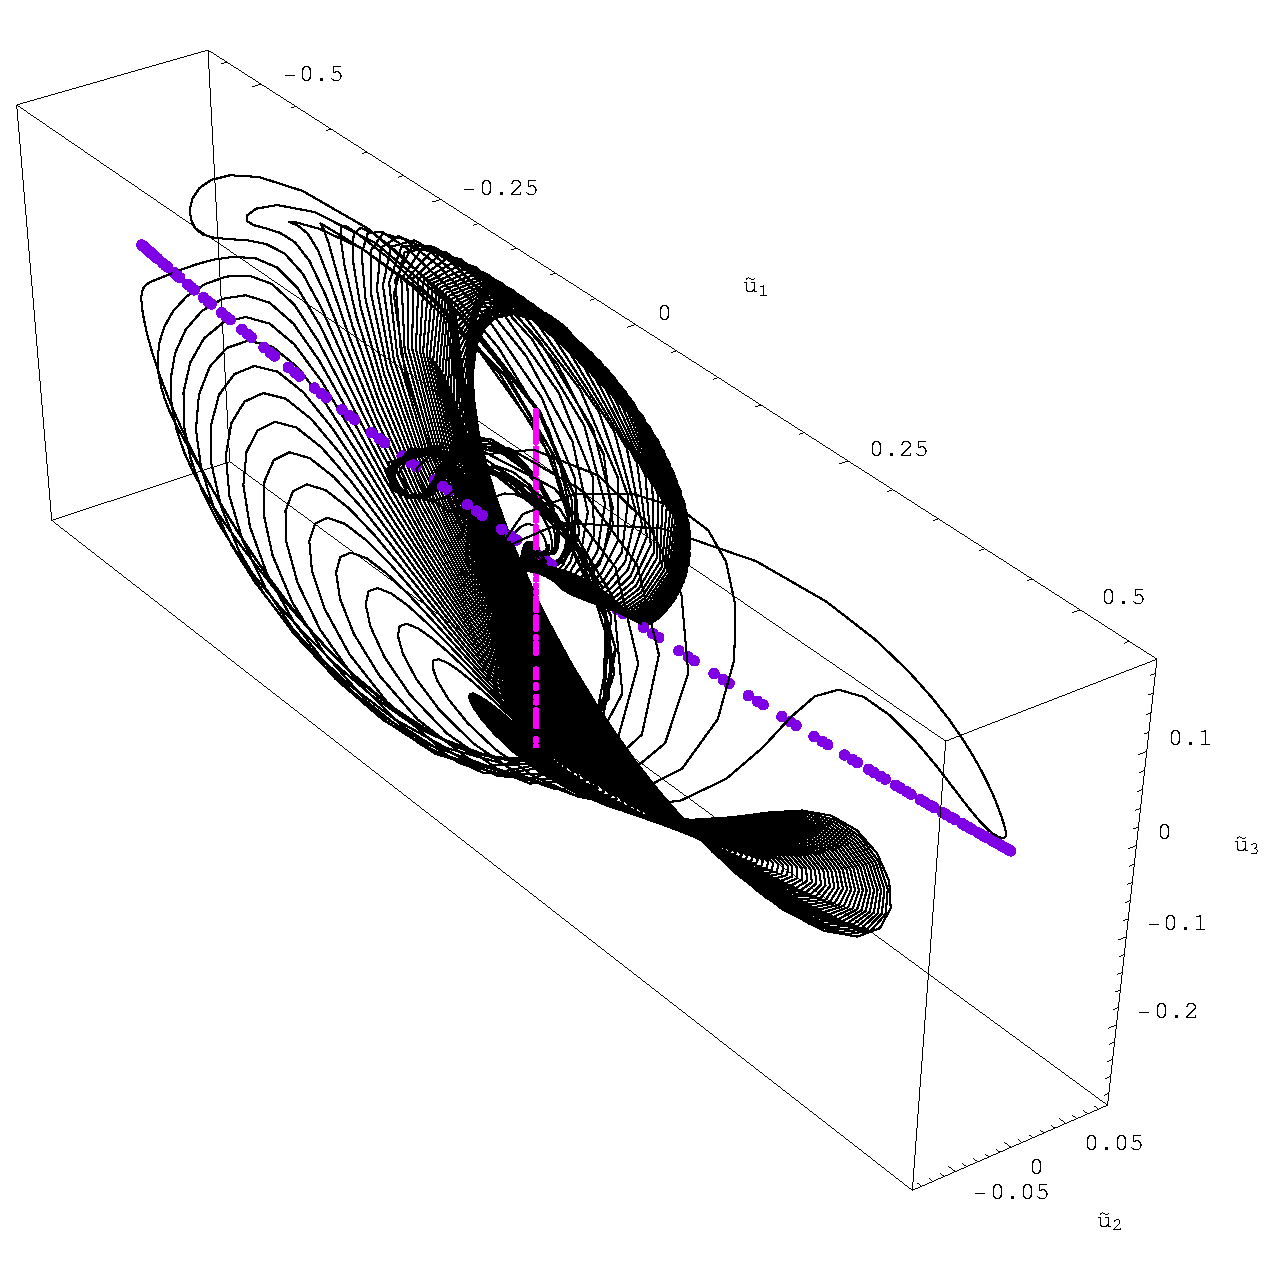
\includegraphics[width=5.0cm]{figs/L22-2w-UnsMan.eps}
\hspace{0.1in}
(b) 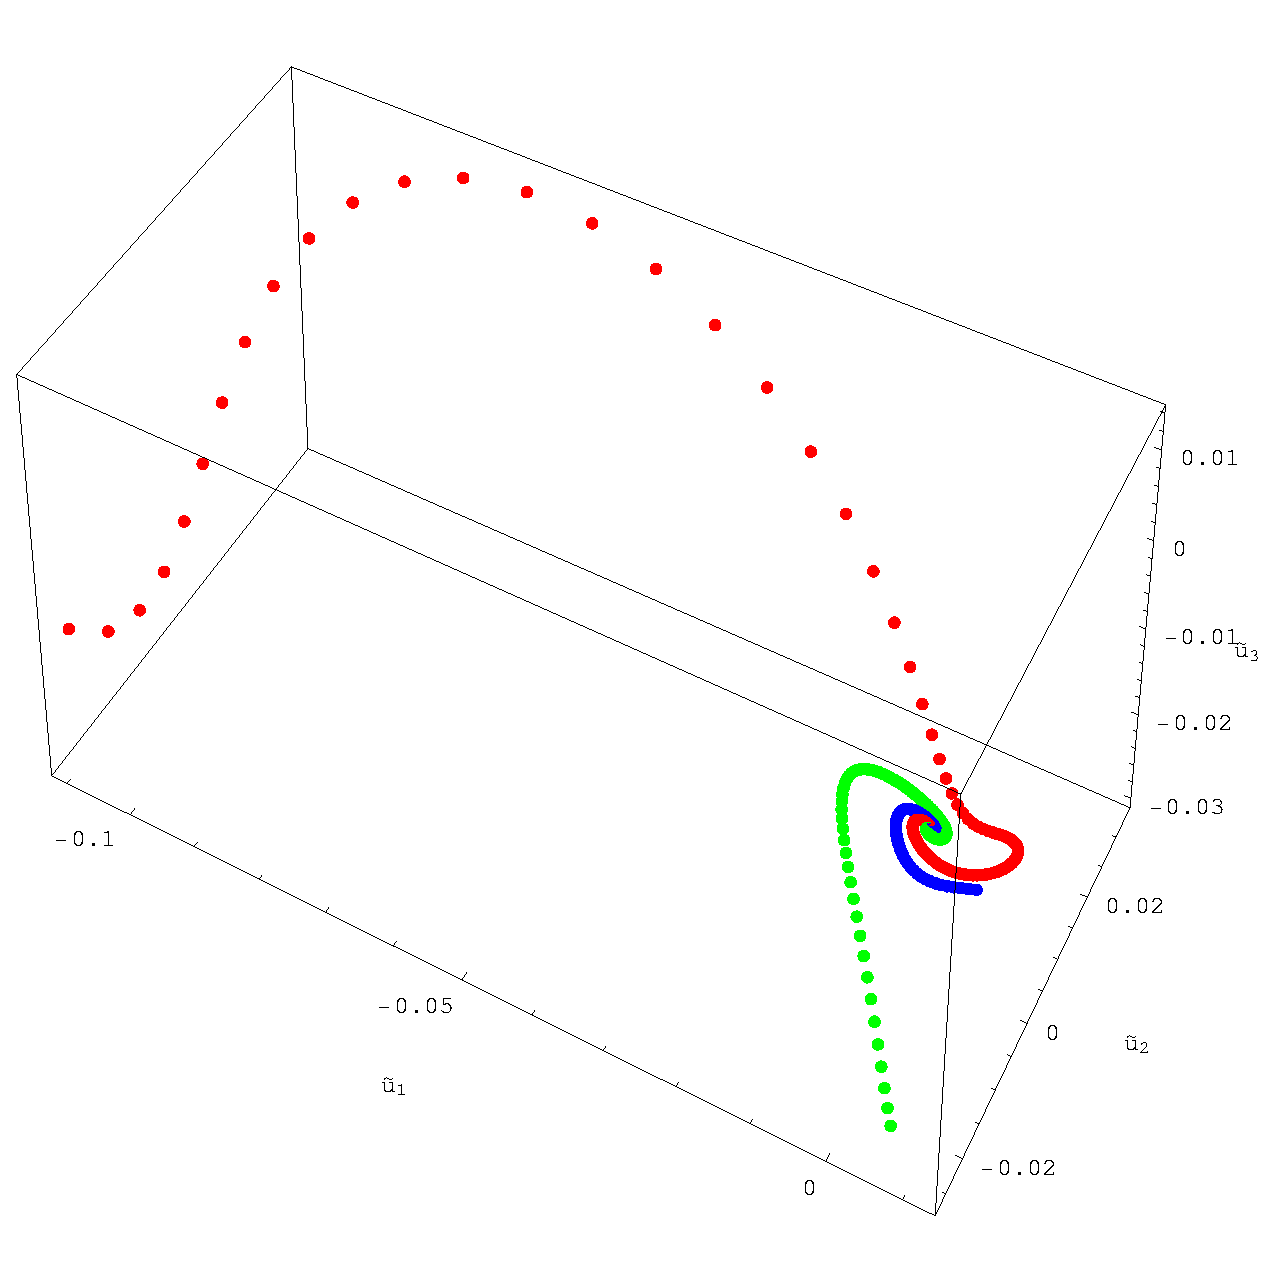
\includegraphics[width=5.0cm]{figs/L22-2w-UnsMan-BlowUp.eps}
% (b) 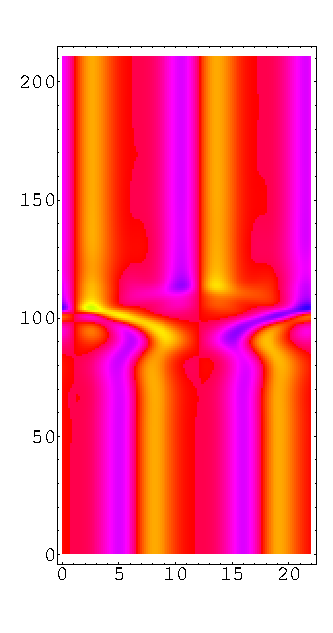
\includegraphics[width=4.0cm]{figs/L22-2w-R.eps}
\\
(c) 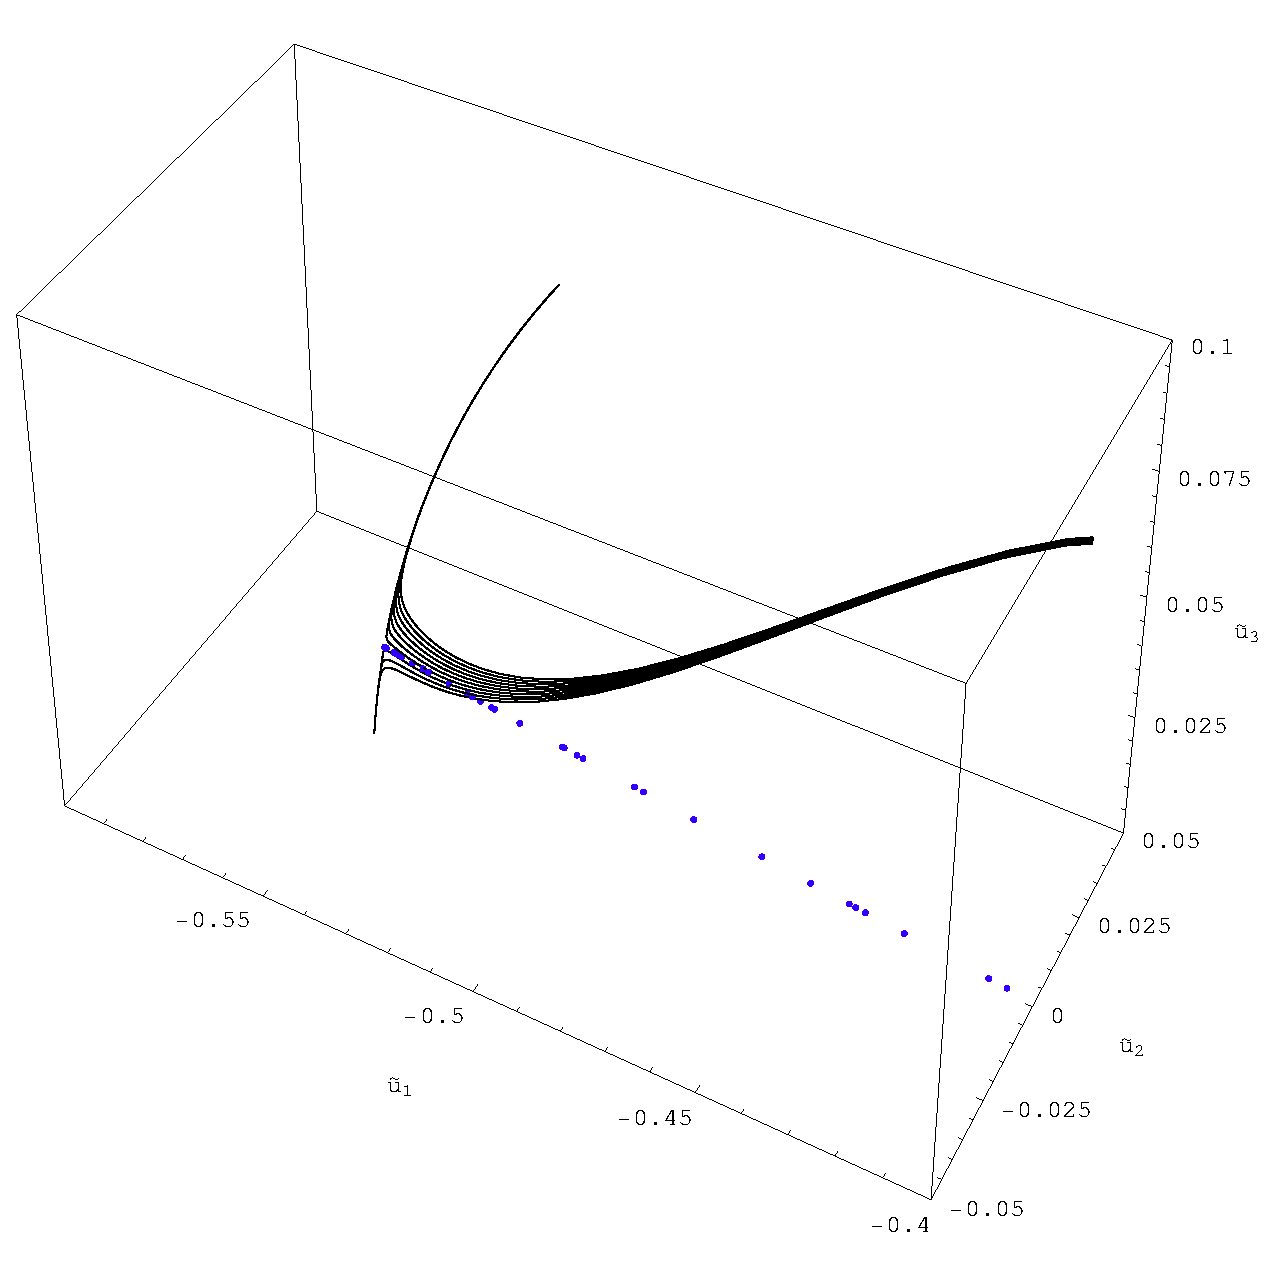
\includegraphics[width=5.0cm]{figs/L22-2w-3w-UnsMan.eps}
% (c) 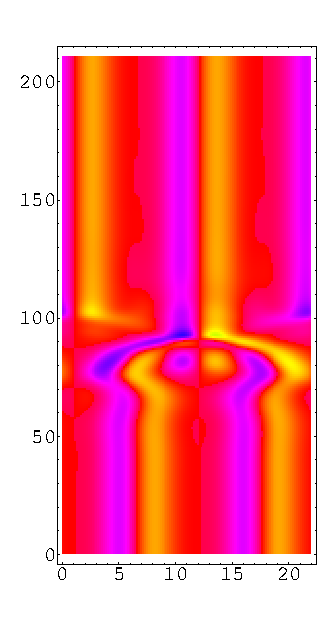
\includegraphics[width=4.0cm]{figs/L22-2w-G.eps}
\hspace{0.1in}
(d)  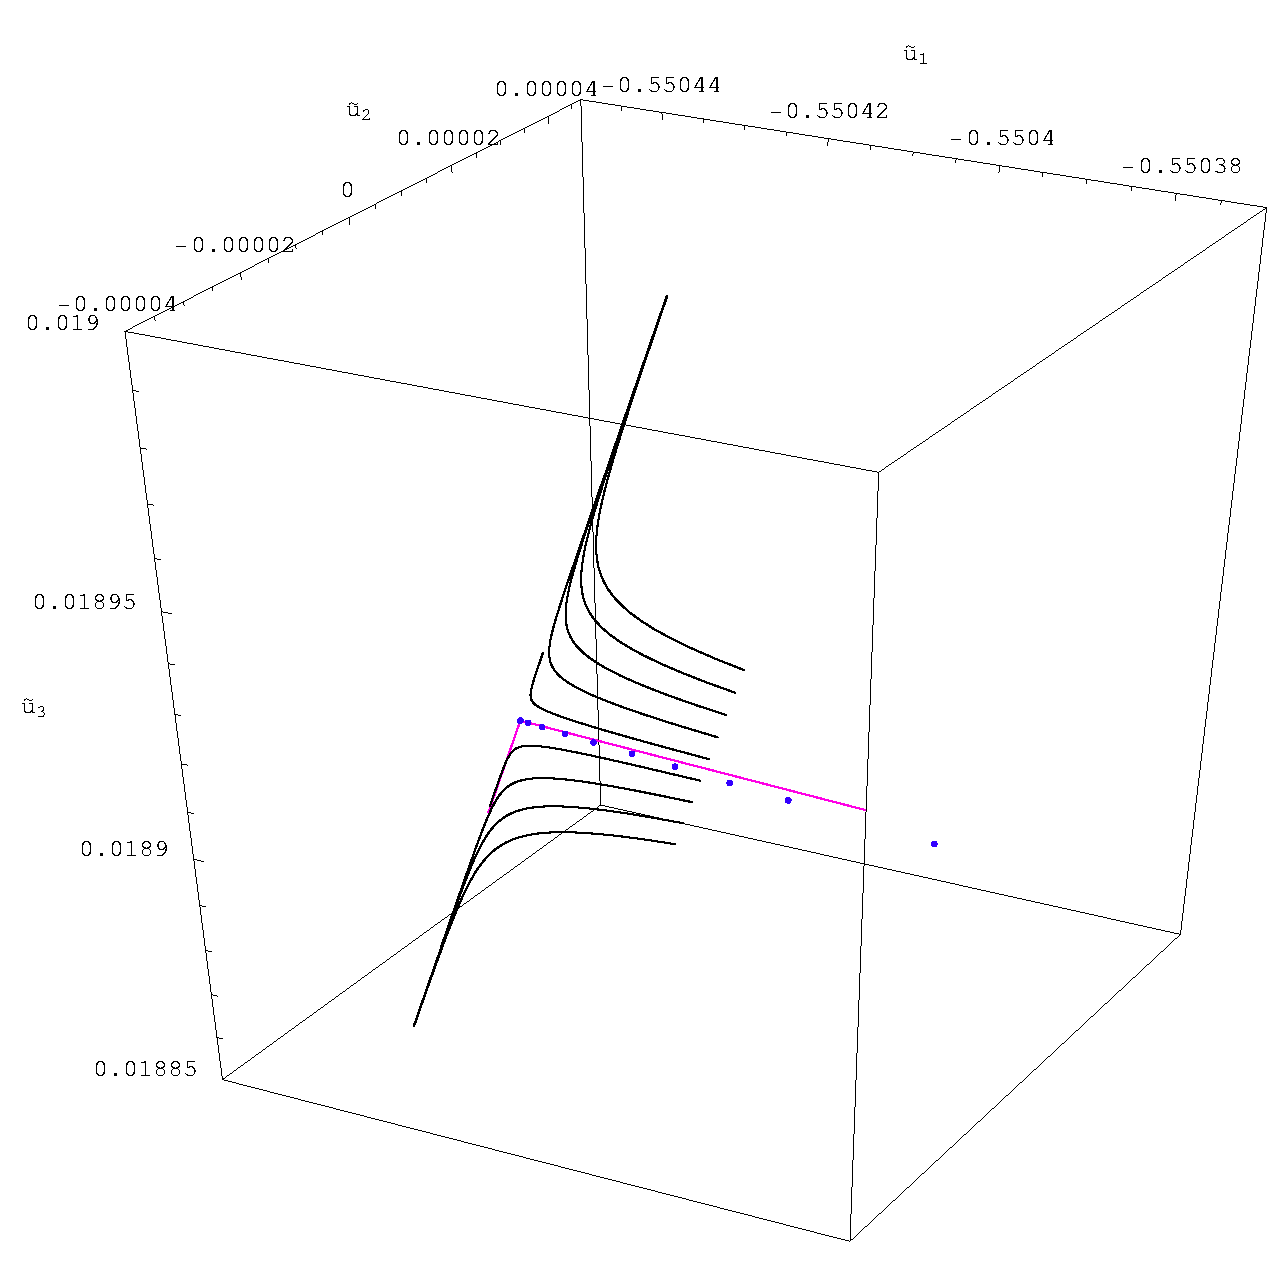
\includegraphics[width=5.0cm]{figs/L22-2w-3w-detail.eps}
% (d) 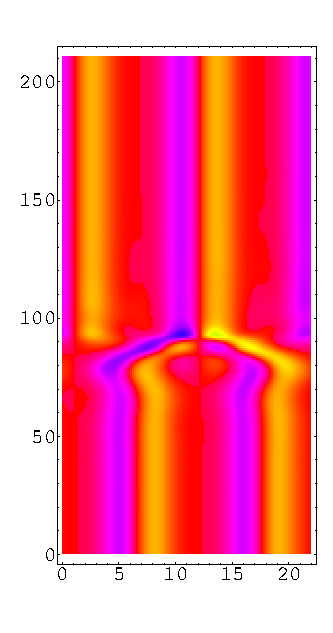
\includegraphics[width=4.0cm]{figs/L22-2w-B.eps}
\caption{
 Trajectories with initial conditions on the unstable subspace of
 the \nameit 2 {\eqva}.
 (a) The coordinates $\tilde{u}_1$ and $\tilde{u}_2$ are along the directions defining the unstable subspace
 and $\tilde{u}_3$  is along the real part of the eigenvector,
 corresponding to the eigenvalue $-0.271122+ i\, 0.356307$. The purple points represent the continous family
 of
\nameit 2 \eqva.
% Green curve belongs to \reffig{f:rpo55}(b) % rpo22-55-4-cm.eps
% rather than to  \reffig{f:rpo55}(a), % rpoEq22-55-4.eps?
(b) blowup of ``homoclinic'' descent of the unstable manifold
back into {\nameit}-2 {\eqv}, shifted by
$L/4 =5.5$.
(c) blowup of ``heteroclinc'' connection from
{\nameit}2 \eqv\ to {\nameit}3 \eqv\, with shift
$L(1/3-1/4) = L/12 = 1.83$ (? check)
to the neighborhood of the point near which the
unstable manifold of the
\nameit 2 \eqv\ splits. The blue points
represent the
\nameit 3 {\eqv} family.
The descent is along the eigenvector of $\Lyap_4= 0.413$ (checked by ES),
and spliting
occurs along one of the
$\Lyap_1=\Lyap_2=0.0933$
unstable directions of the \nameit 2 {\eqv} (checked by ES).
d) same as (c), closer to the \nameit 3 {\eqv}. The eigendirections corresponding to $\Lyap_1$
and $\Lyap_4$ are shown in purple.
}
\label{f:neighborhood2w}
\end{figure}
%%%%%%%%%%%%%%%%%%%%%%%%%%%%%%%%%%%%%%%%%%%%%%%%%%%%%%%%%%%%%%%%%%


\subsection{\Reqva}

In addition to the \eqva\ , the \KS\ system has \reqv\ solutions
(also called traveling or rotating waves in the literature).
They are characterized by a fixed function profile, $u(x)$,
moving with constant speed $c$, i.e.
\[ u(x+ct,t) = u(x, 0)\,,\quad t \in \mathbb{R}\,.\]
Because of the reflection symmetry, the \reqva\ come in pairs
related by the transformation: $u(x) \to -u(-x)$, $c \to -c$.
In Fourier space the \reqva\ are defined by the condition
\[ a_k(t)\mathrm{e}^{-iq_kct} = a_k(0)\,.\]
Differentiating this condition with respect to time, we obtain
equation for the \reqv\
\[ f_k(a) - i q_k c a_k = 0 \]
which needs to be solved for $a_k$ and $c$.

Consistent with the bifurcation diagram of Greene and Kim,
we find two \reqva\ with speeds $c = 0.737$ and $0.350$.
The profiles of the two \reqva\ and their time evolution
with eventual fall into the chaotic attractor are
shown in Figure~\ref{f:ks22tw}.


\underline{1-\reqv\  (traveling wave).}
% Ruslan L Davidchack,  10 Jul 2006
There is a pair of \reqva\
${\nameit}1L$,
${\nameit}1R$
(traveling waves), dual under the
$u(x) \to -u(-x)$ symmetry. They are
determined numerically by
adiabatic continuation from a smaller system size
$L~\approx 12$,
where they are stable, to $L=22$
where their velocity is atypically large, $c=0.737$,

Their exponents are:
\\
$\Lyap_i \pm \theta_i =
(
\\
  0.1156222 \pm 0.817289,   \\
  0.033663 \pm 0.418909,    \\
 0.0                    ,   \\
 -0.245729                    , \\
 -0.321321 \pm 0.98126,
\cdots
)$

The pair of \reqva\
${\nameit}2L$,
${\nameit}2R$
exists for larger system sizes, but does not continue
adiabatically\rf{KNSks90} down to $L=22$.


\subsection{\Eqva, $L$ and $c$}

%%%%%%%%%%%%%%%%%%%%%%%%%%%%%%%%%%%%%%%%%%%%%%%%%%%%%%%%%%%%%%%%
\begin{figure}[t]
    % \vspace*{-5pt}
\centering
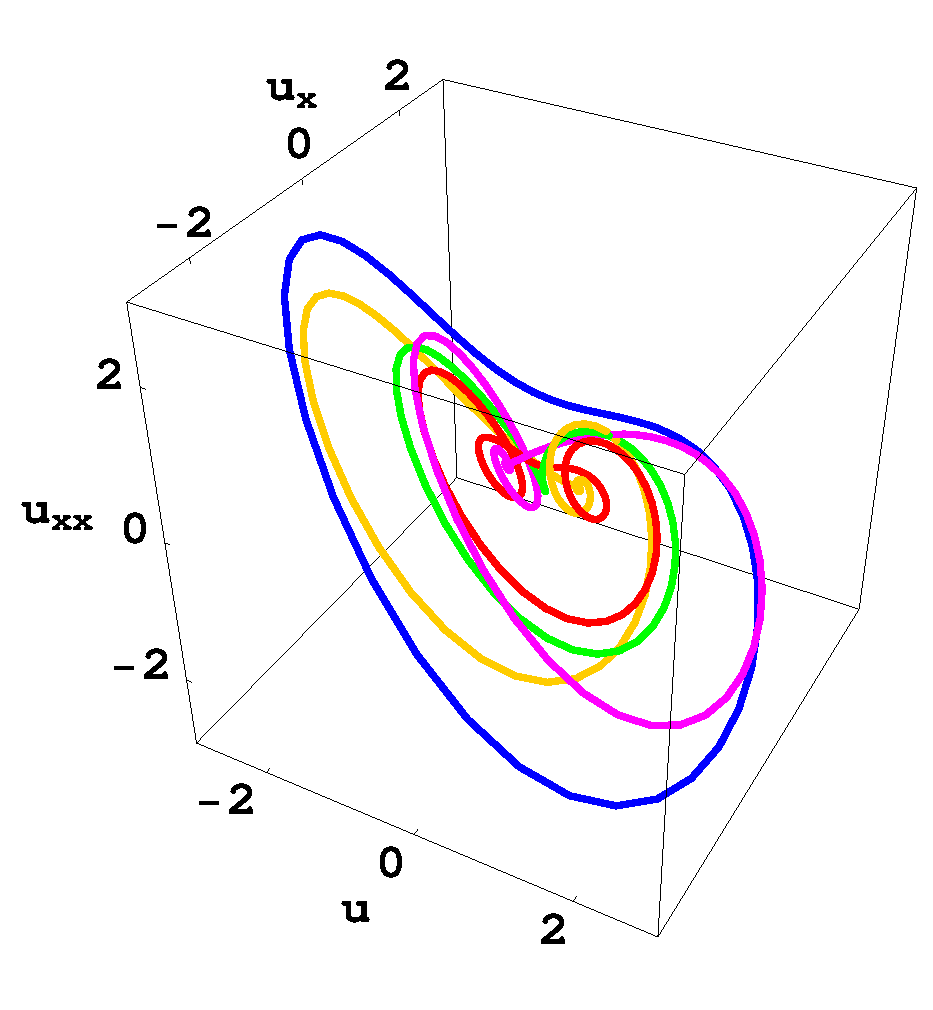
\includegraphics[width=0.6\textwidth]{figs/equilSpatial.eps}
    % \vspace*{-5pt}
\caption{
    {\small
$(u,u_x,u_{xx})$ representation
of $\EQV{1}$ (blue), $\EQV{2}$ (red), $\EQV{3}$ (black) \eqva\ and $\REQV{+}{1}$ (purple), $\REQV{-}{1}$ (orange) \reqva.
$\tildeL=3.5014$, $N=64$ complex modes truncation.
        } %end \small
        }
\label{f:eqvSpatial}
    % \vspace*{-5pt}
\end{figure}
%%%%%%%%%%%%%%%%%%%%%%%%%%%%%%%%%%%%%%%%%%%%%%%%%%%%%%%%%%%%%%%%%%

\PC{
 add the left/right $\REQV{\pm}{1}$ pair to \reffig{f:eqvSpatial}
    }
The $u=0$  \eqv\ $\EQV{0}$ is a point at the origin
in \reffig{f:eqvSpatial}.
At
each integer value of $\tildeL$ the origin spews out a Hopf cycle. That
might help us prove that we have all equilibria for $L=22$.

Each of these \eqva\ has a different value of the $c$ integration
constant.

Plot also the two \eqva\ of \eqva\ points, their
real eigenvectors and their complex eigenplanes. All equilibria presumably
wind around these, and as box size $L$ changes, they form continuous
families with smoothly changing $c$. One can check that by
changing $L$ a bit and using the previous equilibrium to find the next
one.

What does the complex eigenplane continuation does for these
equilibria - does it produce nice heteroclinic connections, or is it
wierder? We know there is an analytic formula for a heteroclinic
connection (see \refref{Lan:Thesis}). % Lan's thesis).

The real motivation for all this is that if we understand \eqva\ as
$L \to \infty$ we might have an entry into $L = \infty$ periodic orbit
theory of KS.

%%%%%%%%%%%%%%%%%%%%%%%%%%%%%%%%%%%%%%%%%%%%%%%%%%%%%%%%%%%%%%%%
\begin{figure}[h]
\centering
(a) 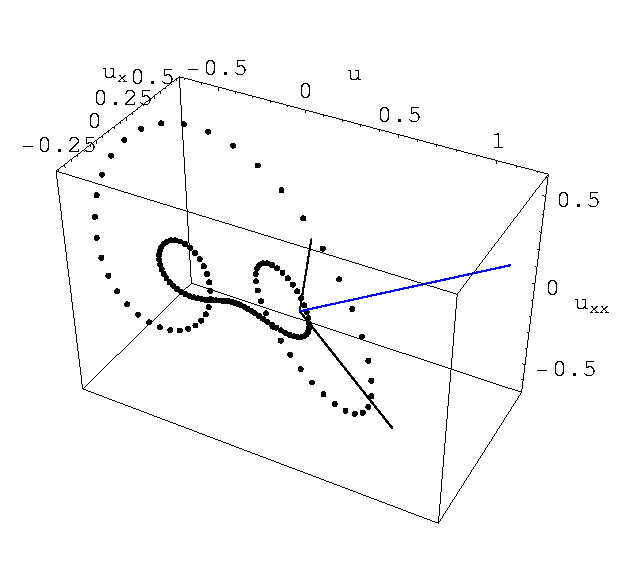
\includegraphics[width=5.0cm]{figs/1wSteadyE.eps}
\hspace{0.1in}
(b) 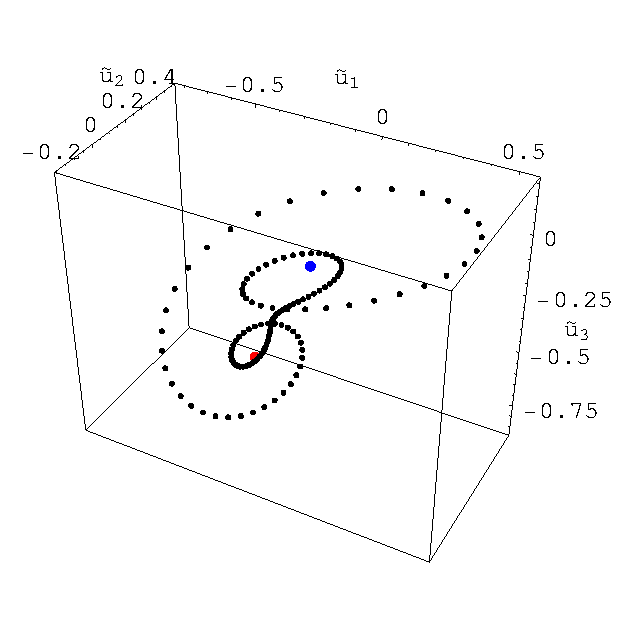
\includegraphics[width=5.0cm]{figs/1wSteadyP.eps}
\caption{
\small{
(a) $\EQV{1}$ in $(u,u_x,u_{xx})$ representation along with the eigenvectors of the equilibrium
point $(\sqrt{c},0,0)$. The blue line represents the unstable eigen-direction.
(b) $\EQV{1}$ projected along the above eigenvectors. $\tildeL=3.5014$, $N=64$ complex modes truncation.
}
}
\label{f:1wSteady}
\end{figure}

\reftab{tab:L22cminus} lists the stability eigenvalues
$\eigExp[1]^-,\eigRe[2]^-\pm\eigIm[2]^-$
of equilibrium point $c_{-}=(-\sqrt{c},0,0)$
of \label{eq:3dks} for $c$ corresponding to each on of $\EQV{1},\EQV{2}$ and $\EQV{3}$ \eqva.
The period of spiraling $T_{-}=2\pi/\theta^-_2$, expansion
rate in the complex plane of spiraling
$\ExpaEig_r\approx\exp(\eigRe[2]^- T_-)$ and contraction
rate along the stable eigendirection
$\ExpaEig_1\approx\exp(\eigRe[1]^- T_-)$ are also listed.

\begin{table}[h!]
% use packages: array
    \begin{tabular}{l|rrrrrr}
                & $E$   &$\eigExp[1]^-$ & $\eigRe[2]^-\pm\eigIm[2]^-$   & $T_m$ & $\ExpaEig_r$  & $\ExpaEig_1$  \\ \hline
        $\EQV{1}\ $ &\ 0.13 &\ -0.55    &\ $0.28\pm1.11i$       &\ 5.67     &\ 4.79     &\ 0.04 \\ \hline
        $\EQV{2}\ $     &\ 0.22 &\ -0.66    &\ $0.33\pm1.15i$       &\ 5.47     &\ 5.99     &\ 0.03 \\ \hline
        $\EQV{3}\ $     &\ 0.79 &\ -0.94    &\ $0.47\pm1.29i$       &\ 4.87     &\ 9.92     &\ 0.01
    \end{tabular}
    \caption{}
    \label{tab:L22cminus}
\end{table}


%%%%%%%%%%%%%%%%%%%%%%%%%%%%%%%%%%%%%%%%%%%%%%%%%%%%%%%%%%%%%%%%%%
